% Options for packages loaded elsewhere
\PassOptionsToPackage{unicode}{hyperref}
\PassOptionsToPackage{hyphens}{url}
\PassOptionsToPackage{dvipsnames,svgnames,x11names}{xcolor}
%
\documentclass[
  letterpaper,
  DIV=11,
  numbers=noendperiod]{scrreprt}

\usepackage{amsmath,amssymb}
\usepackage{lmodern}
\usepackage{iftex}
\ifPDFTeX
  \usepackage[T1]{fontenc}
  \usepackage[utf8]{inputenc}
  \usepackage{textcomp} % provide euro and other symbols
\else % if luatex or xetex
  \usepackage{unicode-math}
  \defaultfontfeatures{Scale=MatchLowercase}
  \defaultfontfeatures[\rmfamily]{Ligatures=TeX,Scale=1}
\fi
% Use upquote if available, for straight quotes in verbatim environments
\IfFileExists{upquote.sty}{\usepackage{upquote}}{}
\IfFileExists{microtype.sty}{% use microtype if available
  \usepackage[]{microtype}
  \UseMicrotypeSet[protrusion]{basicmath} % disable protrusion for tt fonts
}{}
\makeatletter
\@ifundefined{KOMAClassName}{% if non-KOMA class
  \IfFileExists{parskip.sty}{%
    \usepackage{parskip}
  }{% else
    \setlength{\parindent}{0pt}
    \setlength{\parskip}{6pt plus 2pt minus 1pt}}
}{% if KOMA class
  \KOMAoptions{parskip=half}}
\makeatother
\usepackage{xcolor}
\setlength{\emergencystretch}{3em} % prevent overfull lines
\setcounter{secnumdepth}{5}
% Make \paragraph and \subparagraph free-standing
\ifx\paragraph\undefined\else
  \let\oldparagraph\paragraph
  \renewcommand{\paragraph}[1]{\oldparagraph{#1}\mbox{}}
\fi
\ifx\subparagraph\undefined\else
  \let\oldsubparagraph\subparagraph
  \renewcommand{\subparagraph}[1]{\oldsubparagraph{#1}\mbox{}}
\fi


\providecommand{\tightlist}{%
  \setlength{\itemsep}{0pt}\setlength{\parskip}{0pt}}\usepackage{longtable,booktabs,array}
\usepackage{calc} % for calculating minipage widths
% Correct order of tables after \paragraph or \subparagraph
\usepackage{etoolbox}
\makeatletter
\patchcmd\longtable{\par}{\if@noskipsec\mbox{}\fi\par}{}{}
\makeatother
% Allow footnotes in longtable head/foot
\IfFileExists{footnotehyper.sty}{\usepackage{footnotehyper}}{\usepackage{footnote}}
\makesavenoteenv{longtable}
\usepackage{graphicx}
\makeatletter
\def\maxwidth{\ifdim\Gin@nat@width>\linewidth\linewidth\else\Gin@nat@width\fi}
\def\maxheight{\ifdim\Gin@nat@height>\textheight\textheight\else\Gin@nat@height\fi}
\makeatother
% Scale images if necessary, so that they will not overflow the page
% margins by default, and it is still possible to overwrite the defaults
% using explicit options in \includegraphics[width, height, ...]{}
\setkeys{Gin}{width=\maxwidth,height=\maxheight,keepaspectratio}
% Set default figure placement to htbp
\makeatletter
\def\fps@figure{htbp}
\makeatother
\newlength{\cslhangindent}
\setlength{\cslhangindent}{1.5em}
\newlength{\csllabelwidth}
\setlength{\csllabelwidth}{3em}
\newlength{\cslentryspacingunit} % times entry-spacing
\setlength{\cslentryspacingunit}{\parskip}
\newenvironment{CSLReferences}[2] % #1 hanging-ident, #2 entry spacing
 {% don't indent paragraphs
  \setlength{\parindent}{0pt}
  % turn on hanging indent if param 1 is 1
  \ifodd #1
  \let\oldpar\par
  \def\par{\hangindent=\cslhangindent\oldpar}
  \fi
  % set entry spacing
  \setlength{\parskip}{#2\cslentryspacingunit}
 }%
 {}
\usepackage{calc}
\newcommand{\CSLBlock}[1]{#1\hfill\break}
\newcommand{\CSLLeftMargin}[1]{\parbox[t]{\csllabelwidth}{#1}}
\newcommand{\CSLRightInline}[1]{\parbox[t]{\linewidth - \csllabelwidth}{#1}\break}
\newcommand{\CSLIndent}[1]{\hspace{\cslhangindent}#1}

\KOMAoption{captions}{tableheading}
\makeatletter
\makeatother
\makeatletter
\@ifpackageloaded{bookmark}{}{\usepackage{bookmark}}
\makeatother
\makeatletter
\@ifpackageloaded{caption}{}{\usepackage{caption}}
\AtBeginDocument{%
\ifdefined\contentsname
  \renewcommand*\contentsname{Table of contents}
\else
  \newcommand\contentsname{Table of contents}
\fi
\ifdefined\listfigurename
  \renewcommand*\listfigurename{List of Figures}
\else
  \newcommand\listfigurename{List of Figures}
\fi
\ifdefined\listtablename
  \renewcommand*\listtablename{List of Tables}
\else
  \newcommand\listtablename{List of Tables}
\fi
\ifdefined\figurename
  \renewcommand*\figurename{Figure}
\else
  \newcommand\figurename{Figure}
\fi
\ifdefined\tablename
  \renewcommand*\tablename{Table}
\else
  \newcommand\tablename{Table}
\fi
}
\@ifpackageloaded{float}{}{\usepackage{float}}
\floatstyle{ruled}
\@ifundefined{c@chapter}{\newfloat{codelisting}{h}{lop}}{\newfloat{codelisting}{h}{lop}[chapter]}
\floatname{codelisting}{Listing}
\newcommand*\listoflistings{\listof{codelisting}{List of Listings}}
\makeatother
\makeatletter
\@ifpackageloaded{caption}{}{\usepackage{caption}}
\@ifpackageloaded{subcaption}{}{\usepackage{subcaption}}
\makeatother
\makeatletter
\@ifpackageloaded{tcolorbox}{}{\usepackage[many]{tcolorbox}}
\makeatother
\makeatletter
\@ifundefined{shadecolor}{\definecolor{shadecolor}{rgb}{.97, .97, .97}}
\makeatother
\makeatletter
\makeatother
\ifLuaTeX
  \usepackage{selnolig}  % disable illegal ligatures
\fi
\IfFileExists{bookmark.sty}{\usepackage{bookmark}}{\usepackage{hyperref}}
\IfFileExists{xurl.sty}{\usepackage{xurl}}{} % add URL line breaks if available
\urlstyle{same} % disable monospaced font for URLs
\hypersetup{
  pdftitle={Jackknife Variance Estimator for Datasets Containing Multiply Imputed Outcome Variables Under Uncongeniality: A Monte Carlo Simulation Study},
  colorlinks=true,
  linkcolor={blue},
  filecolor={Maroon},
  citecolor={Blue},
  urlcolor={Blue},
  pdfcreator={LaTeX via pandoc}}

\title{Jackknife Variance Estimator for Datasets Containing Multiply
Imputed Outcome Variables Under Uncongeniality: A Monte Carlo Simulation
Study}
\author{}
\date{}

\begin{document}
\maketitle
\ifdefined\Shaded\renewenvironment{Shaded}{\begin{tcolorbox}[borderline west={3pt}{0pt}{shadecolor}, breakable, frame hidden, sharp corners, enhanced, boxrule=0pt, interior hidden]}{\end{tcolorbox}}\fi

\renewcommand*\contentsname{Table of contents}
{
\hypersetup{linkcolor=}
\setcounter{tocdepth}{2}
\tableofcontents
}
\bookmarksetup{startatroot}

\hypertarget{title-page}{%
\chapter*{\texorpdfstring{{Title Page}}{Title Page}}\label{title-page}}

A Thesis

Presented to the Department of Mathematics and Statistics

Hal Marcus College of Science and Engineering

and

The Kugelman Honors Program

of

The University of West Florida

In partial fulfillment of the requirements for graduation as a Kugelman
Honors Scholar

Ihsan E. Buker

November, 2022

\bookmarksetup{startatroot}

\hypertarget{acknowledgments}{%
\chapter*{Acknowledgments}\label{acknowledgments}}

I would like to thank my cat.

\bookmarksetup{startatroot}

\hypertarget{abstract}{%
\chapter{Abstract}\label{abstract}}

Missing data is an issue ubiquitous in many fields of science. Today,
multiple imputation (MI) is one of the most commonly utilized approaches
to provide valid statistical inferences in the presence of missing data.
Briefly, MI fills the missing cells in the original dataset by
generating a series of plausible values based on an imputation model
and, thereafter, creates multiple complete versions of the original
dataset. Subsequently, the analysis model is applied to each imputed
dataset, and the parameters of interest are pooled to accurately reflect
the loss of information caused by the missing observations. Accompanying
MI is the issue of uncongeniality, which occurs when the imputation
model and the analysis model make different assumptions about the data.
Not long after the conception of MI, Rubin's accompanying set of rules
to pool parameter estimates from the multiply imputed datasets was shown
to produce biased point estimates under uncongeniality, which led to
under-coverage of confidence intervals for anti-conservative estimates
of variance or over-coverage for conservative estimates. In response,
certain combinations of MI and resampling methods have been proposed as
robust variance estimators under uncongeniality; however, their main
drawback, to this day, has been their associated computational cost.
Moreover, bootstrapping, one of the most commonly utilized resampling
methods alongside MI to obtain proper variance estimates, has its basis
in asymptotic theory. As such, in small samples frequently encountered
in biological studies, the need for a computationally efficient variance
estimator with statistically desirable properties remains.

In response, a jackknife variance estimator for multiply imputed outcome
variables under uncongeniality for small sample sizes is proposed, which
provides asymptotically unbiased point estimates with appropriate
confidence interval coverage under uncongeniality. The performance of
the proposed jackknife variance estimator is investigated using a Monte
Carlo simulation study and compared to other methods in the literature.
Accordingly, the recommendation to replace Rubin's rules as the de facto
standard in variance estimation with resampling-based robust variance
estimators is made, particularly in light of the modern computational
power statistical practitioners have at their disposal. Finally, an
implementation of the proposed jackknife variance estimator in R is
provided.

\hypertarget{keywords}{%
\section{Keywords}\label{keywords}}

Multiple imputation, uncongeniality, model misspecification, jackknife
resampling

\bookmarksetup{startatroot}

\hypertarget{background}{%
\chapter{Background}\label{background}}

Missing data is a discipline-agnostic issue commonly encountered by
statistical practitioners. Given that many statistical procedures
require data to be complete (i.e., in the form of an \(n \times m\)
matrix), the appropriate course of action to be taken in the presence of
missing data has long been investigated by statisticians. Today,
multiple imputation is accepted as the gold standard in missing data
analysis, thanks to the work of Donald Rubin {[}1{]}. In 1977, Rubin
proposed using multiple completed versions of the dataset with missing
observations, applying the complete-data procedure of interest, and
pooling the estimates to draw valid inferences {[}1{]}. The main
advantage of multiple imputation, as opposed to single imputation, which
had been used by researchers since the early 1970s, is its ability to
properly estimate the variance caused by missing observations {[}1{]}.
The emphasis placed on variance and uncertainty by Rubin was a departure
from the status quo of the time, which was to fill in the missing
observation with the most probable value and to proceed with complete
case analyses as if the observation had not been missing, to begin with
{[}1{]}. This approach, however, fails to incorporate the loss of
information caused by missing observations into the estimation of
parameters, resulting in the underestimation of variance {[}2{]}.

Like all revolutionary ideas, multiple imputation received harsh
criticism following its conception. Perhaps the most notable of the
objections came from Fay in 1992, who demonstrated through
counterexamples that multiple imputation produced biased covariance
estimates {[}3{]}. Fay added that the need for unison between the
imputation and analysis model made multiple imputation a poor
general-purpose tool, particularly in instances where the imputer and
analyst are different individuals {[}1{]}, {[}4{]}. Fay's arguments led
to the conceptualization of congeniality\footnote{Please see the
  appendix for a detailed overview of congeniality.} between the
imputation and analysis model, which was later accepted to be a
requirement to obtain valid inferences from multiple imputation using
Rubin's pooling rules (hereafter, Rubin's rules) {[}1{]}, {[}5{]}.
Briefly, uncongeniality refers to the imputation and analysis model
making irreconcilably different assumptions regarding the data, which
occurs rather frequently in practice {[}3{]}. Although Fay's work
initially criticized biases introduced to the covariance matrix
following multiple imputation, a similar phenomenon of biased estimates
were observed with variance estimators under uncongeniality
{[}4{]}--{[}6{]}.

Some of the earliest works demonstrating Rubin's variance estimator to
be biased under uncongeniality were from Wang and Robins in 1998, who
also proposed an alternate variance estimator in the same paper {[}1{]}.
The variance estimator proposed by Wang and Robins requires the
calculation of several quantities, which are not easily accessible to
the average statistical practitioner {[}3{]}. The challenging
construction of the variance estimator proposed by Wang and Robins has
resulted in it receiving little-to-no attention in applied settings
{[}3{]}. In an attempt to create a more user-friendly variance estimator
in instances of suspected uncongeniality, researchers have proposed
combining resampling methods with multiple imputation. Of the two main
resampling methods, bootstrap has received more attention from multiple
imputation researchers compared to jackknife resampling, which has
mostly been investigated under single hot-deck imputation. Although
particular combinations of bootstrap and multiple imputation have been
demonstrated to create asymptotically unbiased estimates of variance,
the associated computational cost makes this an active area of research
{[}3{]}. Most recently, von Hippel has proposed a bootstrap variance
estimator which addresses the issue of computational cost; however, it
has been demonstrated to create confidence intervals that are slightly
wider compared to traditional bootstrap and multiple imputation
combinations {[}3{]}. Given the lower computational cost associated with
jackknife resampling, as well as desirable properties demonstrated under
single imputation, such as being unbiased in certain scenarios, it is an
attractive alternative that should be considered as a variance estimator
of multiply imputed data under uncongeniality {[}7{]}, {[}8{]}. More
importantly, however, is the advantages jackknife resampling has over
bootstrap resampling in small sample sizes, which are frequently
encountered in datasets associated with biological studies.

\hypertarget{bootstrap-resampling}{%
\section{Bootstrap Resampling}\label{bootstrap-resampling}}

Let \(q\) be the set of observations
\(\left(z_1, z_2, z_3, \dots, z_n \right)\) from the population \(Q\)
such that \(z_i \ \forall \ i \in \{1, 2, 3, \dots, n\}\) is an
i.i.d\footnote{i.i.d stands for independent and identically distributed,
  which is used to summarize two characteristics about the data; (1)
  that the samples are all taken from the same probability distribution,
  and (2) that the samples are obtained independently.} sample from
\(Q\). Moreover, let \(\theta\) be some parameter of interest, with the
unbiased estimator \(\hat{\theta}\), which is a statistic computed from
\(F(q)\). Finally, let \(G_{\theta}\) be the sampling distribution of
\(F(q)\). The non-parametric bootstrap, as proposed by Efron, lets \(q\)
define \(Q\) such that the set of observations
\(\left(z_1, z_2, z_3, \dots, z_n \right)\) appears with equal
proportion in the infinitely large population. From there, the set of
samples \(q^*_1, q^*_2, q^*_3, \dots, q^*_m\) as
\(m \rightarrow \infty\) are generated by sampling \(n\) observations
with replacement from \(q\), and the statistic of interest
\(\hat{\theta}\) is calculated by applying
\(F(q_i) \ \forall \ i \in \{1, 2, 3, \dots, m\}\), which results in
\(\hat{\theta^*}_1, \hat{\theta^*}_2, \hat{\theta^*}_3, \dots, \hat{\theta^*}_m\).

Finally, the point estimate is obtained by

\[\hat{\theta} = m^{-1}\sum^m_{i = 1} \hat{\theta^*}_i\]

and the variance is obtained by

\[\text{var}(\hat{\theta}) = m^{-1}\sum^m_{i = 1} \left(\hat{\theta^*}_i - \hat{\theta}\right)^2\]

Since Efron's proposal of the non-parametric bootstrap, statisticians
have widely utilized it thanks to its ease of implementation and the
rapidly increasing computational power available to statistical
practitioners {[}9{]}. However, the properties of bootstrap resampling
have their basis in the asymptotic theory, which holds in large sample
sizes {[}10{]}, {[}11{]}. The minimum sample size required to utilize
bootstrap resampling and obtain asymptotically unbiased estimates is
highly context-dependent; in certain situations, a minimum sample size
of \(n = 200\) has been suggested, with other authors suggesting between
\(n = 100\) to \(n = 500\) {[}12{]}--{[}14{]}. Given that in many
biological studies, the minimum sample size required for asymptotically
unbiased estimates may not be achieved, jackknife resampling, a method
that predates the bootstrap, may be considered {[}15{]}.

\hypertarget{jackknife-resampling}{%
\section{Jackknife Resampling}\label{jackknife-resampling}}

\hypertarget{sec-del}{%
\subsection{Leave-One-Out Jackknife}\label{sec-del}}

Let \(q\) be the set of observations
\(\left(z_1, z_2, z_3, \dots, z_n \right)\) from the population \(Q\)
such that \(z_i \ \forall \ i \in \{1, 2, 3, \dots, n\}\) is an i.i.d
sample from \(Q\). Moreover, let \(\theta\) be some parameter of
interest, with the unbiased estimator \(\hat{\theta}\), which is a
statistic computed from \(F(q)\). Finally, let \(G_{\theta}\) be the
sampling distribution of \(F(q)\). The jackknife, as proposed by
Quenouille and expanded on by Tukey, creates \(n\) leave-one-out
subsamples from \(q\) such that
\(q_{-1} = \left(z_2, z_3, z_4, \dots, z_n \right),\)
\(q_{-2} = \left(z_1, z_3, z_4, \dots, z_n \right), \dots, q_{-n} = \left(z_1, z_2, z_3, \dots, z_{n-1} \right)\)
and \(\lvert q_{-i}\rvert = n-1 \ \forall i \in \{1, 2, 3, \dots, n\}\).
Thereafter, the statistic of interest \(\hat{\theta}\) is calculated by
applying \(F(q_i) \ \forall \ i \in \{1, 2, 3, \dots, n\}\), which
results in
\(\hat{\theta^*}_1, \hat{\theta^*}_2, \hat{\theta^*}_3, \dots, \hat{\theta^*}_m\).

Finally, the point estimate is obtained by

\[
\hat{\theta} = n^{-1}\sum^n_{i = 1} \hat{\theta^*}_i
\]

and the variance is obtained by

\[
\text{var}(\hat{\theta}) = n^{-1}\sum^n_{i = 1} \left(\hat{\theta^*}_i - \hat{\theta}\right)^2
\]

\hypertarget{delete-d-jackknife}{%
\subsection{\texorpdfstring{Delete-\emph{d}
Jackknife}{Delete-d Jackknife}}\label{delete-d-jackknife}}

The delete-\emph{d} jackknife may be seen as a generalized version of
the traditional jackknife (hereinafter, jackknife). Although in many
situations, the jackknife provides a computationally efficient means to
estimate the variance of an estimator, it fails with non-smooth
statistics. For non-smooth statistics, such as the percentiles of the
data, the jackknife fails because the statistic varies significantly
between any two subsamples {[}7{]}. In such cases, the delete-\emph{d}
jackknife provides an alternative estimator that can provide
asymptotically unbiased estimates for non-smooth statistics {[}8{]}.
Similarly, let \(q\) be the set of observations
\(\left(z_1, z_2, z_3, \dots, z_n \right)\) from the population \(Q\)
such that \(z_i \ \forall \ i \in \{1, 2, 3, \dots, n\}\) is an i.i.d
sample from \(Q\). Moreover, let \(\theta\) be some parameter of
interest, with the unbiased estimator \(\hat{\theta}\), which is a
statistic computed from \(F(q)\). Finally, let \(G_{\theta}\) be the
sampling distribution of \(F(q)\). The delete-\emph{d} jackknife,
creates \(n \choose d\) subsamples of \(q\) such that
\(\lvert q_i \rvert = n-d\) Thereafter, the statistic of interest
\(\hat{\theta}\) is calculated by applying
\(F(q_i) \ \forall \ i \in \{1, 2, 3, \dots, {n \choose d} \}\), which
results in
\(\hat{\theta^*}_1, \hat{\theta^*}_2, \hat{\theta^*}_3, \dots, \hat{\theta^*}_{n \choose d}\).
In many cases, however, \(n \choose d\) is a large value that yields
this approach computationally unfeasible. In such instances, certain
guidelines, as discussed in following chapters, may be employed to
determine a value of subsamples that still provide proper estimates.

Finally, the point estimate is obtained by

\[ 
\hat{\theta} = {n \choose d}^{-1}\sum^{n \choose d}_{i = 1} \hat{\theta^*}_i
\]

and the variance is obtained by

\[
\text{var}(\hat{\theta}) = {n \choose d}^{-1}\sum^{n \choose d}_{i = 1} \left(\hat{\theta^*}_i - \hat{\theta}\right)^2
\]

\hypertarget{comparison-of-jackknife-and-bootstrap-resampling}{%
\section{Comparison of Jackknife and Bootstrap
Resampling}\label{comparison-of-jackknife-and-bootstrap-resampling}}

Given their comparable construction and application, the jackknife and
bootstrap make similar assumptions regarding the data. Most notably,
both assume that the function used to estimate the parameter is smooth.
Formally, a smooth function is defined as one that has continuous
derivatives over some domain, with the minimum number of derivatives
required to be considered smooth varying per the question at hand
{[}16{]}. From a statistical perspective, if the function used to
estimate the parameter is smooth on some domain \((a, b)\),
\([F(q_i) - F(q_z)] \rightarrow 0\) as
\(\lvert q_i - q_z\rvert \rightarrow 0\). Meaning, among a set of
conceivable, non-identical samples from the population, minor
differences between possible samples will only result in minor
differences between the statistic estimated {[}7{]}. Due to its
deterministic nature, the jackknife tends to perform poorly in
estimating non-smooth statistics {[}17{]}. However, its deterministic
nature also yields the jackknife superior to bootstrapping in smaller
datasets. To combat the issue regarding non-smooth statistics, a
generalized jackknife resampling scheme, called the
\emph{drop-d-jackknife} has been proposed, which was utilized in this
estimator {[}7{]}.

\hypertarget{multiple-imputation}{%
\section{Multiple Imputation}\label{multiple-imputation}}

Multiple imputation is a missing data management method based on both
Bayesian and frequentist inference proposed by Donald Rubin in the late
1970s {[}1{]}, {[}3{]}. Before Rubin's proposal, statisticians had been
utilizing various single-imputation methods and proceeding with the
analyses of interest as if data had not been missing. However, Rubin
noted that single-imputation methods could not accurately capture the
uncertainty caused by the missing observations {[}1{]}. In response, he
proposed imputing any given datum with a series of plausible values from
its posterior distribution, thus creating several complete versions of
the observed dataset and applying the complete data analysis procedure
to each generated dataset. He proposed a series of rules that could
derive point and variance estimates that would adequately reflect the
uncertainty caused by the missing observations.

Rubin's idea to utilize multiple imputation was ridiculed at first, not
only due to its drastically different interpretation of uncertainty but
because of how unfeasible it was at the time {[}1{]}. Rubin's method
would require statisticians to come up with an imputation model that
would allow them to draw values from the posterior distribution. After
that, they would have to draw several values and repeat the analysis
multiple times with the numerous complete datasets. The preceding
workflow was challenging to implement in an era of low computational
power and expensive digital storage {[}1{]}. As such, Rubin's ideas did
not receive immediate acceptance. However, since the late 1990s, with
the increased access to computers and user-friendly statistical packages
capable of implementing complex procedures, multiple imputations have
been adopted and heavily researched, leading to various modified
algorithms being utilized under different conditions to obtain valid
inferences in the presence of missing data {[}1{]}. At this time, one of
the most notable challenges remaining with multiple imputation is the
concept of congeniality. Congeniality may be thought of as the
imputation model and the analysis model making compatible assumptions
regarding the data. In the early 1990s, Fay and Meng demonstrated that
congeniality was required to obtain valid inferences from multiple
imputation {[}3{]}, {[}18{]}.

\hypertarget{current-state-of-multiple-imputation}{%
\subsection{Current State of Multiple
Imputation}\label{current-state-of-multiple-imputation}}

Today, with the advent of public databases, the imputer and the analyst
may no longer be the same person. Even in the absence of such cases, the
imputation and analysis model may still be uncongenial if there does not
exist a unifying Bayesian model which embeds the imputer's imputation
model and the analyst's complete data procedure {[}18{]}. As such,
researchers have begun to develop approaches that combine resampling
methods with multiple imputation to obtain valid inferences even under
uncongeniality. Of the currently proposed methods, there exist two main
limitations: a) the increased computational cost brought on by
resampling methods alongside multiple imputation, and b) inference in
smaller sample sizes. At this time, nearly all mainstream approaches
proposed by researchers utilize bootstrap resampling and multiple
imputation to obtain valid inferences under uncongeniality; however, as
discussed above, bootstrap resampling requires a certain sample size to
provide proper estimates. As a viable alternative to be utilized in
instances where there is a small sample size, a jackknife variance
estimator is proposed.

\bookmarksetup{startatroot}

\hypertarget{methods}{%
\chapter{Methods}\label{methods}}

For the proposed Monte Carlo simulation, \(N\) = 10,000 datasets were
generated with the following characteristics: A response variable,
\(Y\), where 30\% of the observations were missing at random
(MAR)\footnote{Please see the appendix for a detailed overview of
  mechanisms of missingness, and their implications.}, and an
\(n \times q\) matrix of fully observed covariates, where \(n = 50\) was
the sample size, and \(q = 3\) the number of covariates.

Formally

\[
\begin{bmatrix} V1 \\V2 \\ V3 \end{bmatrix} \sim N\left(\begin{bmatrix} 1\\ 1 \\ 1 \end{bmatrix}, \begin{bmatrix} 1 & 0.5 & 0.5 \\
0.5 & 1 & 0.5 \\
0.5 & 0.5 & 1
\end{bmatrix}\right)
\]

With

\[
\beta_{V_1} = 2 ; \  \beta_{V_2} = 5 ; \ \beta_{V_3} = 8
\]

The outcome variable was simulated such that:

\[
Y = V_1 + V_2 + V_3 + \epsilon
\]

Where

\[
\epsilon \sim N(\mu = 0, \sigma \propto V_2)
\]

Thus, data were simulated with heteroskedastic errors, which yields the
imputation and analysis models congenial, yet misspecified.

Formally, the analysis model of interest was

\[
\widehat{Y} \sim \widehat{\beta}_{V_1} + \widehat{\beta}_{V_2} + \widehat{\beta}_{V_3} 
\]

And the imputation model was

\[
\widehat{Y}_{\text{mis}} \sim \widehat{\beta}_{V_1} + \widehat{\beta}_{V_2} + \widehat{\beta}_{V_3}
\]

Where the imputation method of choice was predictive mean matching
(PMM).

All generated datasets were analysed using three approaches:

\begin{itemize}
\item
  \textbf{Bootstrap then multiply impute:} The observed dataset with
  missing observations was initially bootstrapped \(n = 200\) times.
  Thereafter, each of the bootstrap samples were imputed \(m = 2\)
  times, with a maximum of \(maxit = 5\) iterations. The mean of the
  bootstrap estimates served as the final point estimate, and a 95\%
  confidence interval was generated through the percentile method, where
  the \(\alpha/2^{th}\) and \(1-(\alpha/2)^{th}\) percentiles were the
  lower and upper bounds, respectively. The R package, \emph{bootImpute}
  was utilized for this process.
\item
  \textbf{Multiply impute then use Rubin's rules:} The observed dataset
  with missing observations was imputed \(m = 10\) times, with a maximum
  of \(maxit = 5\) iterations. The point estimate, as well as the
  confidence interval was obtained through the following rules proposed
  by Donald Rubin. The \emph{mice} package was utilized for this
  process.
\end{itemize}

\begin{align}
\bar{\theta} &= \frac{1}{m}\left (\sum_{i=1}^m{\theta_i}\right ) \\ 
V_{\text{within}} &= \frac{1}{m} \sum_{i=1}^m{SE_i^2} \\ 
V_{\text{between}} &= \frac{\sum_{i=1}^m (\theta_i - \overline{\theta})^2}{m-1} \\ 
V_{\text{total}} &= V_W + V_B + \frac{V_B}{m} \\ 
\bar{\theta} &\pm t_{df,1-\alpha/2} * \sqrt{V_{\text{total}}} 
\end{align}

\begin{itemize}
\tightlist
\item
  \textbf{Jackknife then multiply impute:} Although a more detailed
  overview of the proposed jackknife estimator is provided in
  Chapter~\ref{sec-est}, briefly, the observed dataset was jackknifed to
  obtain \(j = 200\) samples, each of which were imputed \(m = 2\)
  times, with a maximum of \(maxit = 5\) iterations. The mean of the
  jackknife estimates served as the final point estimate, and a 95\%
  confidence interval was generated through the percentile method, where
  the \(\alpha/2^{th}\) and \(1-(\alpha/2)^{th}\) percentiles were the
  lower and upper bounds, respectively.
\end{itemize}

Thereafter, the methods examined were compared concerning their point
estimates, confidence intervals, and computational expense.

All analyses were be conducted using R 4.2.1 (Funny-Looking Kid).

\bookmarksetup{startatroot}

\hypertarget{sec-est}{%
\chapter{The Proposed Jackknife Estimator}\label{sec-est}}

A pseudocode overview of the jackknife estimator proposed may be seen in
the following figure.

\begin{figure}

{\centering 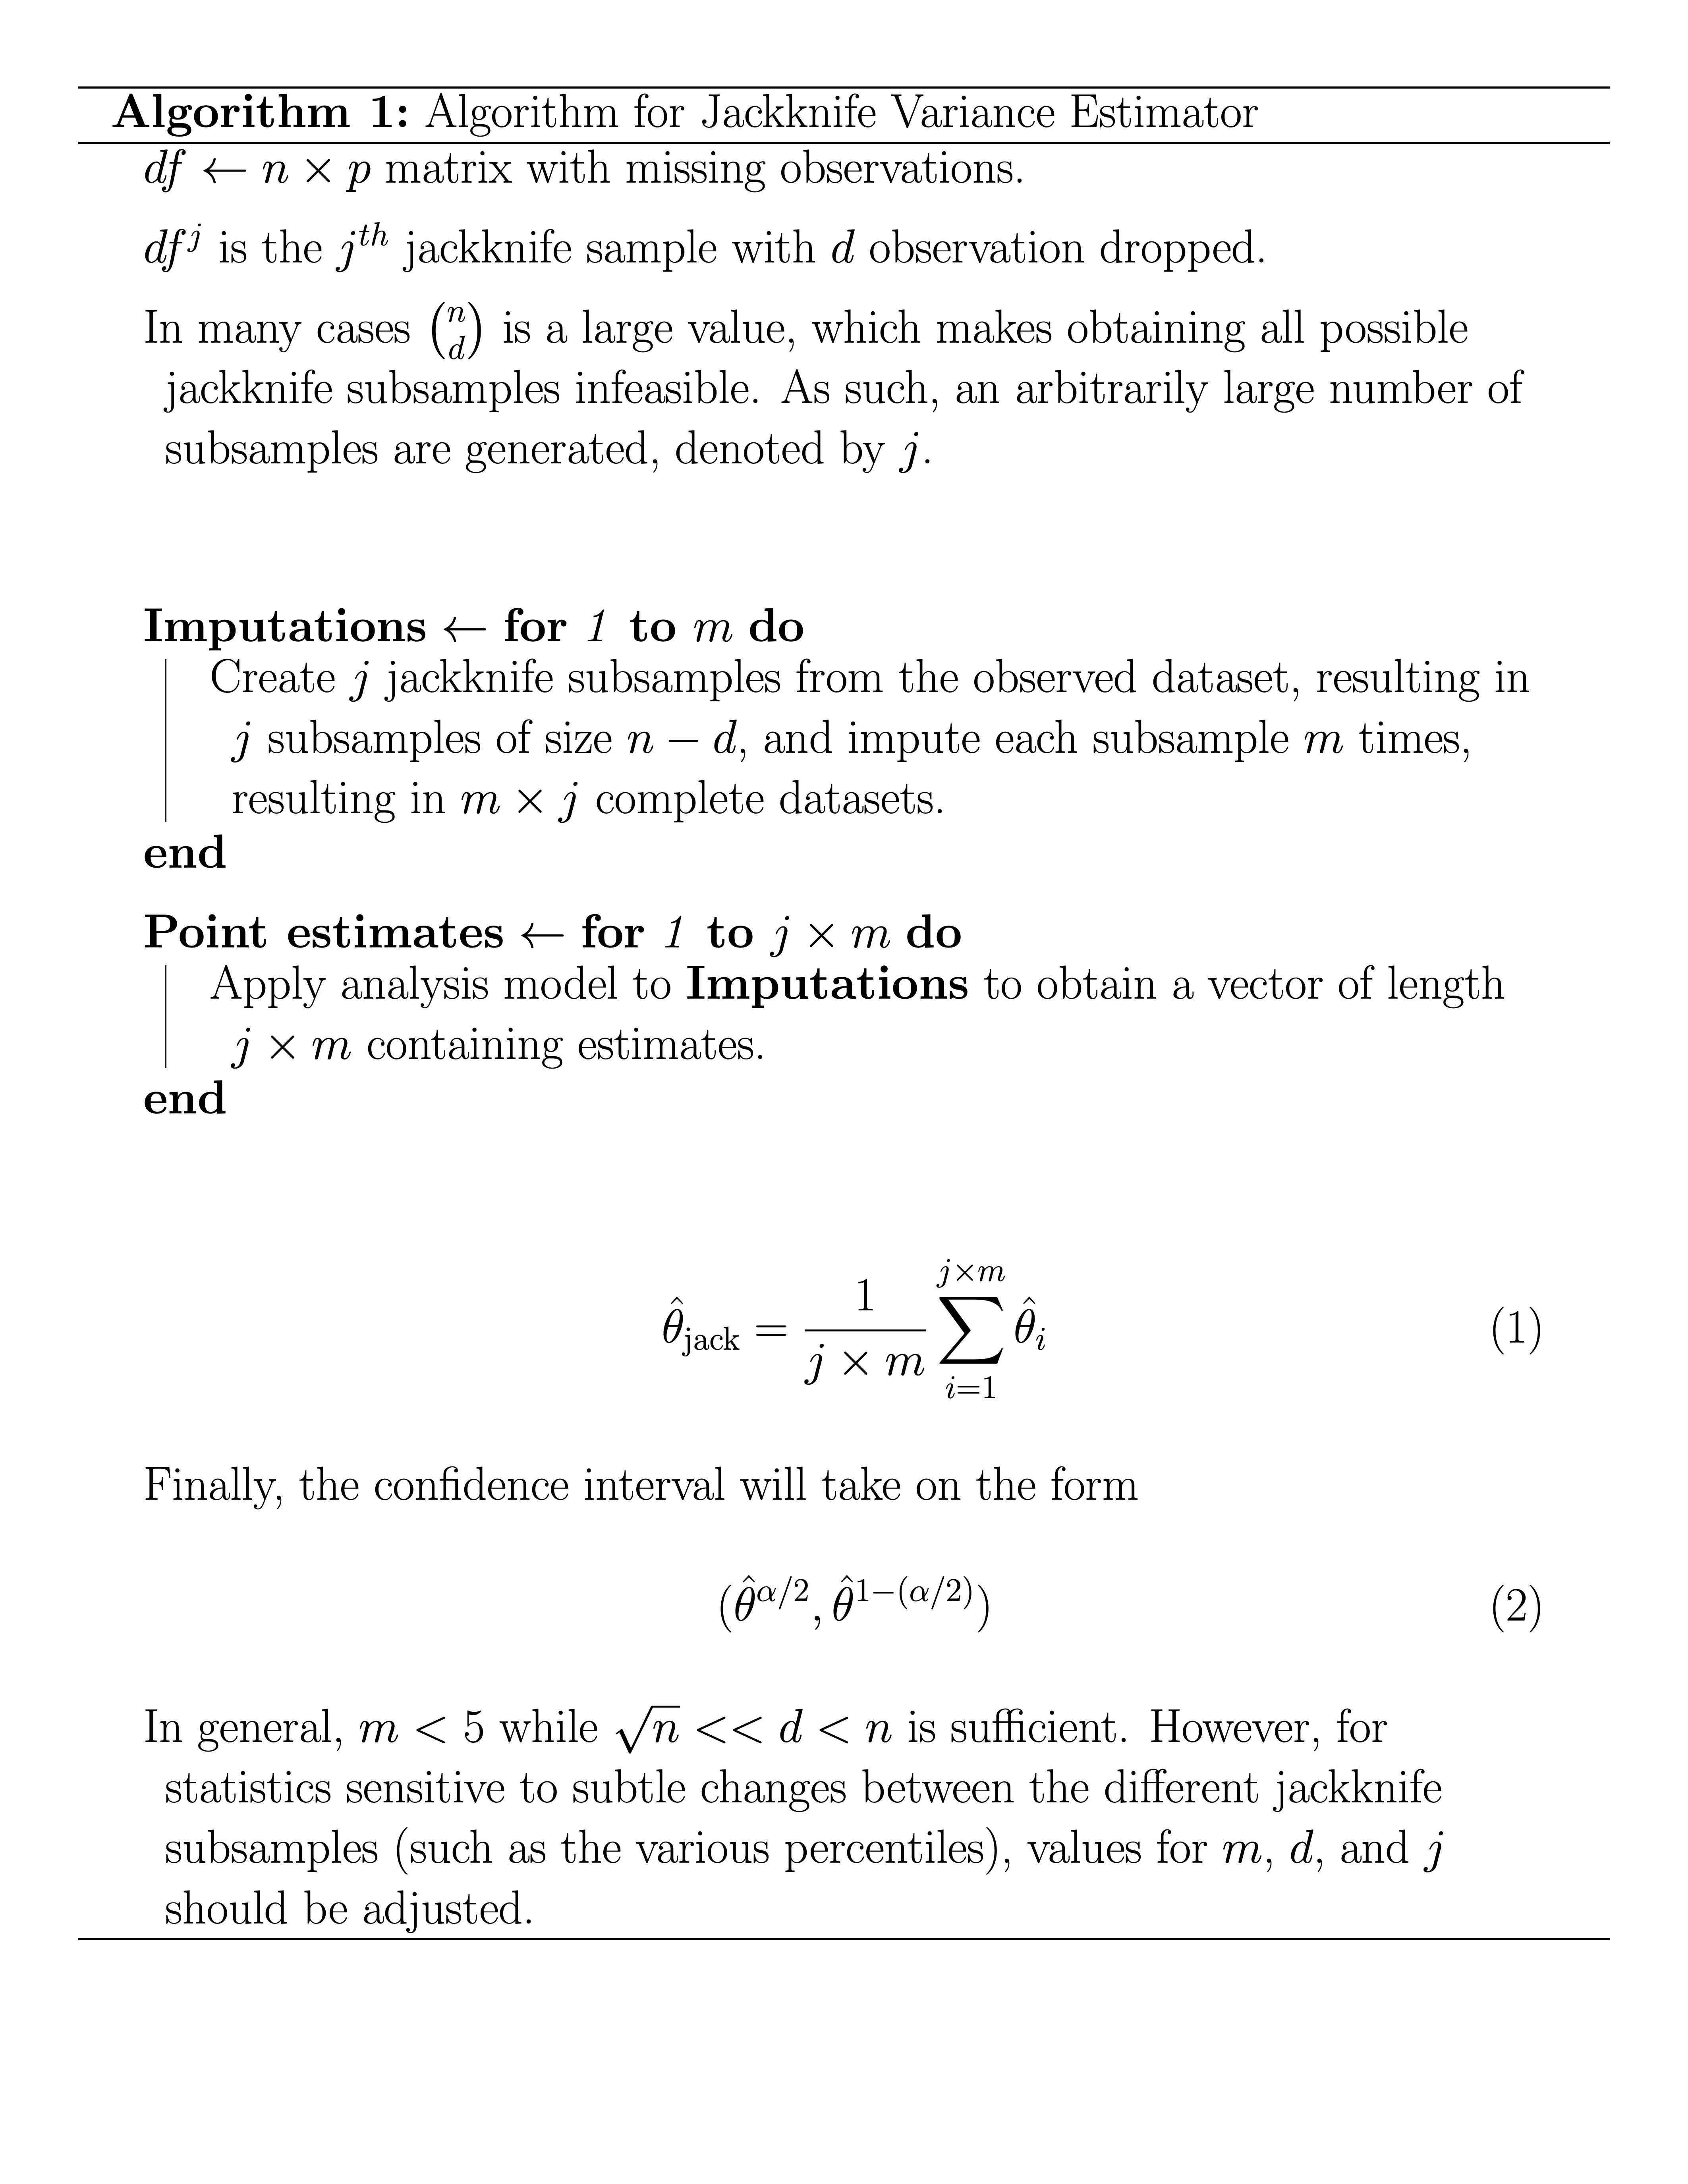
\includegraphics{./Algorithm_for_jackknife_estimator.jpg}

}

\caption{A pseudocode depiction of the proposed estimator.}

\end{figure}

Briefly, the algorithm begins by obtaining \(j\) jackknife subsamples
from the observed dataset with missing observations. Thereafter, each of
the \(j\) subsamples are imputed \(m\) times, resulting in a total of
\(j \times m\) complete datasets. Subsequently, the analysis model of
interest to estimate \(\theta\) is applied to each of the completed
datasets to produce
\(\hat{\theta^*}_1, \hat{\theta^*}_2, \hat{\theta^*}_3, \dots, \hat{\theta^*}_{n \choose d}\).
The point estimate then becomes the mean of the previously produced
\(n\) pseudo-estimates. As for the confidence interval, the
\(\alpha/2^{th}\) and \(1-\alpha/2^{th}\), values serve as the lower and
upper bounds, respectively.

As part of the algorithm, researchers must choose values \(d\) and
\(j\), which will be context-dependent quantities. Ideally, a \(d\)
value which satisfies \(\frac{\sqrt{n}}{d} \rightarrow 0\) will provide
asymptotically unbiased estimates even for non-smooth statistics
{[}7{]}, {[}19{]}. Rewriting the foregoing condition for \(d\)

\begin{align}
&\frac{\sqrt{n}}{d} \rightarrow \ 0 \\ 
&\implies d >> \sqrt{n} \\ 
&\text{Since} \ n > d \\
&\implies n > d >> \sqrt{n}
\end{align}

It is evident that \(d\) should take on some value between \(n\) and
\(\sqrt{n}\) with \(d\) being closer to \(n\), particularly for
non-smooth statistics. At any rate, \(j = {n \choose d}\) will likely be
a value that is not computationally feasible to obtain. As such, the
number of subsamples required, \(j\), can be limited to yield the
estimator more accessible. The choice of \(j\) will be a multifaceted
decision, where, if possible, greater values are preferred. Ideally, a
small pilot study may be performed with a range of \(j\) values to
determine values of \(j\) for which estimates begin to converge.

Although not as widely applicable, researchers may consider utilizing a
delete-one jackknife, as discussed in Section~\ref{sec-del} Given the
stochastic nature of multiple imputation, especially in instances where
a high proportion of missingness is present, the pseudo-estimates may
vary widely between any two given jackknife subsamples, similar to what
would be observed in the case of percentiles. As such, the delete-one
jackknife approach is not recommended for general use but could be
considered in samples with low missingness proportion.

\bookmarksetup{startatroot}

\hypertarget{results}{%
\chapter{Results}\label{results}}

Per the Methods section, the performance of the proposed jackknife
estimator was compared to two leading methods in the literature, Rubin's
rules following multiple imputation and Bootstrap resampling prior to
multiple imputation. The methods were compared concerning the coverage
probabilities they generated, the widths of their respective confidence
intervals, their computational expense, and the bias of their point
estimators.

\hypertarget{point-estimates}{%
\section{Point Estimates}\label{point-estimates}}

All methods, perhaps with the exception of Rubin's rules, produced
reasonable point estimates with minimal bias. Rubin's rules resulted in
slightly anticonservative point estimates with greater standard
deviation, indicative of a statistically inefficient estimator with high
variability. This finding is unsurprising given the literature on
Rubin's rules and its performance under uncongeniality.

In contrast, it is noted that both resampling methods examined provide
nearly unbiased point estimates with smaller standard deviations
compared to Rubin's rules. Again, given the literature on
uncongeniality, this finding was unsurprising; however, given the lack
of both empirical and theoretical justification for the bootstrap
approach in small sample sizes, the desirable properties noted are
worthy of further examination. Between all three methods, nevertheless,
it is noted that the proposed jackknife estimator produced estimates
with the smallest amount of bias, as well as the smallest standard
deviation, an observation perhaps better observed in
Section~\ref{sec-dist}, where the distribution of the biases of the
point estimates is compared. From the kernel density plots presented, it
is evident that Rubin's rules slightly underestimate the parameter.
Compared to Rubin's rules, both resampling approaches provide point
estimates that are nearly unbiased; however, it is noted that the
bootstrap estimates, despite being centered near zero, are slightly more
dispersed compared to the jackknife estimates, which present as a narrow
distribution centered at zero. This observation is justified by the
values provided in Section~\ref{sec-point} which demonstrate that the
jackknife point estimates have a smaller standard deviation than the
bootstrap approach and Rubin's rules.

From a point estimation perspective, the statistically desirable
properties of the jackknife estimator, alongside its theoretical and
empirical justification when used with small sample sizes, yield it a
desirable estimator.

\hypertarget{sec-point}{%
\subsection{Summary of Point Estimation Properties}\label{sec-point}}

\begin{tabular}{lrrr}
\toprule
Method & Median Point Estimates  & Mean Point Estimates & SD of Point Estimates\\
\midrule
Jackknife & 1.971975 & 1.965713 & 0.3648634\\
Bootstrap & 1.928350 & 1.921044 & 0.4442088\\
Rubin's Rules & 1.788012 & 1.750637 & 0.4962010\\
\bottomrule
\end{tabular}

\hypertarget{sec-dist}{%
\subsection{Distribution of Point Estimator Bias}\label{sec-dist}}

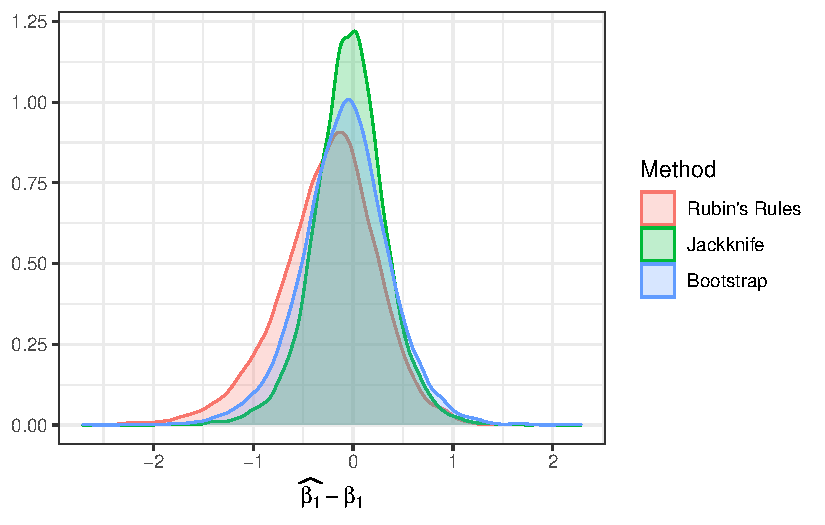
\includegraphics{./results_files/figure-pdf/unnamed-chunk-3-1.pdf}

\hypertarget{sec-ci}{%
\section{Confidence Intervals}\label{sec-ci}}

Over-coverage of confidence intervals is noted across all methods;
however, particulary with the jackknife and bootstrap approaches, such
over-coverage is only slightly over the nominal, as such, they are
likely not of concern and can be explained, in part, by the Monte Carlo
standard error for the true coverage proabability of a 95\% confidence
interval. Among the three methods noted, Rubin's rules, by a significant
margin, deviates from the nominal coverage, indicative of an overly
conservative estimator. An argument could be made, particulary in the
case of biological studies that an overly conservative estimator is
safer than one that is anti-conservative; however, the statistical
inefficieny created by conservative estimators can be of concern,
particulary in instances where small sample sizes are present or the
test being utilized already has low statistical power. Comparing these
methods concerning confidence interval width, it is noted that both
resampling approaches provide narrower confidence intervals, with the
jackknife approach providing the narrowest confidence intervals by a
wide margin. In instances where nominal, or near-nominal coverage is
reached, narrower confidence intervals are indicative of more efficient
estimators. Given the near-nominal coverage noted with the jackknife
estimator, combined with the narrow confidence intervals it produces,
its superiority to the two other methods may be inferred.

A visual overview of the coverage probabilities may be noted in
Section~\ref{sec-zip}, where zipper plots of the methods are presented
utilizing a simple random sample of 100 observations from the Monte
Carlo simulation results of all methods examined. Given the small number
of subsamples examined for visual clarity, the plots may not be
indicative of the larger results presented above; however, they provide
an appreciation for the meaning of coverage probabilities.

\begin{tabular}{lrrrr}
\toprule
Method & Coverage Probability & Median C.I. Width & Mean C.I. Width & SD of C.I. Width\\
\midrule
Jackknife & 97.67 & 1.610436 & 1.683248 & 0.5197257\\
Bootstrap & 97.69 & 2.161853 & 2.228137 & 0.6423704\\
Rubin's Rules & 98.46 & 2.455640 & 2.537168 & 0.7230490\\
\bottomrule
\end{tabular}

\hypertarget{sec-zip}{%
\subsection{Zipper Plots for Confidence Interval
Coverage}\label{sec-zip}}

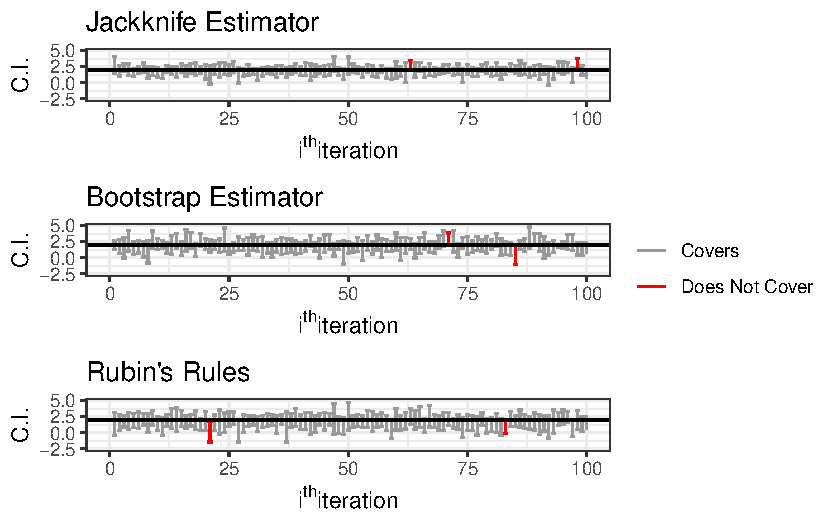
\includegraphics{./results_files/figure-pdf/unnamed-chunk-5-1.pdf}

\hypertarget{performance-benchmark-results}{%
\section{Performance Benchmark
Results}\label{performance-benchmark-results}}

Finally, the three methods are compared concerning their computational
expenses. Comparing the two approaches, which require further
resampling, it is noted that the bootstrap approach takes nearly ten
times longer than the jackknife approach per iteration. Unsurprisingly,
Rubin's rules, which do not rely on any further resampling besides the
one performed during multiple imputation, was the fastest approach.
However, given its biased estimates under uncongeniality or
misspecification, the computational advantage it brings to the table
adds very little value.

Despite generating the same number of subsamples \((n = 200)\), albeit
in contrasting manners, with the same number of imputations \((m = 2)\)
and iterations \((maxit = 5)\), it is surprising that the bootstrap
approach took nearly ten times longer per iterations to provide
estimates. Regardless, the significantly reduced computational expense
of the jackknife estimator yields it superior to the bootstrap approach
under this particular scenario.

\begin{tabular}{lrrr}
\toprule
Method & Median Time (seconds/iteration) & Mean Time (seconds/iteration) & SD of Time (seconds/iteration)\\
\midrule
Jackknife & 8.658003 & 8.800480 & 0.6319727\\
Bootstrap & 72.480187 & 73.012739 & 1.6246321\\
Rubin's Rules & 3.188039 & 3.183781 & 0.0913400\\
\bottomrule
\end{tabular}

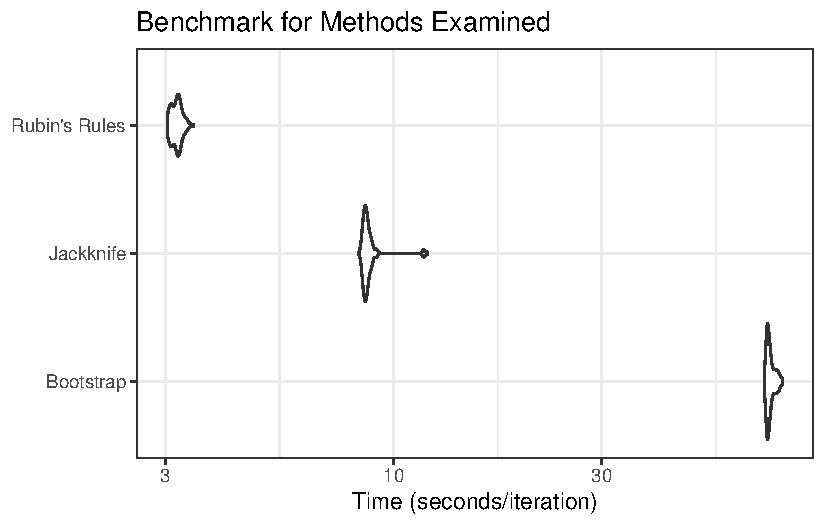
\includegraphics{./results_files/figure-pdf/unnamed-chunk-7-1.pdf}

\bookmarksetup{startatroot}

\hypertarget{discussion}{%
\chapter{Discussion}\label{discussion}}

\hypertarget{conclusion}{%
\section{Conclusion}\label{conclusion}}

In this paper, a jackknife estimator for multiply imputed outcome
variables under the concern of uncongeniality was presented. The
proposed estimator was compared to two alternative approaches in the
literature employing a Monte Carlo simulation study, where all methods
were evaluated on the bias of their point estimates, the width and
coverage of their confidence intervals, and computational time. All
procedures were found to slightly over-cover, suggesting conservative
variance estimates, with Rubin's rules resulting in the broadest
confidence intervals with significant over-coverage compared to the
nominal level. In contrast, the two resampling-based approaches examined
resulted in a substantial decline in confidence interval width, with the
proposed jackknife estimator providing the narrowest confidence
intervals by a wide margin while still attaining near-nominal coverage.

Unsurprisingly, Rubin's rules were the least computationally costly
approach among the ones examined; however, given its downward-biased
point estimates and wide confidence intervals, particularly in instances
where uncongeniality is a concern, resampling-based robust methods
should be preferred. Among the two resampling-based methods examined,
the bootstrap approach took nearly ten times longer per iteration, which
was a surprising observation, as both the jackknife and bootstrap
methods utilized the same number of imputations, iterations, and
subsamples. From a computational perspective, there is no evident reason
why the bootstrap method should take nearly ten times longer than the
proposed jackknife estimator. It is possible that the R package utilized
for the bootstrap approach, \emph{bootImpute}, is not optimized with
speed concerns in mind. However, neither was the jackknife estimator. In
both instances, the most time-consuming aspect of the processes was the
imputation of the subsamples generated, either via bootstrap resampling
or jackknife resampling, done with the same R package, \emph{mice}, and
the same parameters, number of iterations, and imputations. Given that
the foregoing steps took place under identical conditions, perhaps a
different aspect of the two approaches could explain the discrepancy
noted.

Nevertheless, given the superior performance of the jackknife estimator
noted, alongside its computational efficiency, the recommendation to
replace Rubin's rules as the de facto standard in small, multiply
imputed datasets with our proposed estimator is made.

\hypertarget{future-directions}{%
\section{Future Directions}\label{future-directions}}

Perhaps the most significant issue noted with the jackknife estimator
was a slightly higher coverage probability compared to the nominal.
Although the Monte Carlo error may partially explain this observation,
alternative confidence interval construction approaches could be
considered to yield more appropriate coverage. Namely, it is possible
that a confidence interval could be generated by examining various
values calculated based on Rubin's rules, such as the fraction of
missing information, relative efficiency, and relative increase in
variance. The aforestated statistics could be used to appropriately
model the uncertainty in the imputation process, which, in turn, could
be used to generate confidence intervals in a semi-parametric manner.

Otherwise, although the proposed estimator was efficient even with a
small number of subsamples and imputations, alternative confidence
interval constructions could allow one to utilize even fewer subsamples
while still attaining nominal coverage, which may make the proposed
method even more computationally feasible.

\bookmarksetup{startatroot}

\hypertarget{references}{%
\chapter*{References}\label{references}}
\addcontentsline{toc}{chapter}{References}

\hypertarget{refs}{}
\begin{CSLReferences}{0}{0}
\leavevmode\vadjust pre{\hypertarget{ref-buuren_flexible_2012}{}}%
\CSLLeftMargin{{[}1{]} }%
\CSLRightInline{S. van Buuren, \emph{Flexible imputation of missing
data}. Boca Raton, {FL}: {CRC} Press, 2012.}

\leavevmode\vadjust pre{\hypertarget{ref-rubin1978multiple}{}}%
\CSLLeftMargin{{[}2{]} }%
\CSLRightInline{D. B. Rubin, {``Multiple imputations in sample surveys-a
phenomenological bayesian approach to nonresponse,''} in
\emph{Proceedings of the survey research methods section of the american
statistical association}, 1978, vol. 1, pp. 20--34.}

\leavevmode\vadjust pre{\hypertarget{ref-bartlett_bootstrap_2020}{}}%
\CSLLeftMargin{{[}3{]} }%
\CSLRightInline{J. W. Bartlett and R. A. Hughes, {``Bootstrap inference
for multiple imputation under uncongeniality and misspecification,''}
\emph{Stat Methods Med Res}, vol. 29, no. 12, pp. 3533--3546, Dec. 2020,
doi:
\href{https://doi.org/10.1177/0962280220932189}{10.1177/0962280220932189}.}

\leavevmode\vadjust pre{\hypertarget{ref-fay1992inferences}{}}%
\CSLLeftMargin{{[}4{]} }%
\CSLRightInline{R. E. Fay, {``When are inferences from multiple
imputation valid?.''} 1992.}

\leavevmode\vadjust pre{\hypertarget{ref-meng_multiple-imputation_1994}{}}%
\CSLLeftMargin{{[}5{]} }%
\CSLRightInline{X.-L. Meng, {``Multiple-imputation inferences with
uncongenial sources of input,''} \emph{Statistical Science}, vol. 9, no.
4, pp. 538--558, Nov. 1994, doi:
\href{https://doi.org/10.1214/ss/1177010269}{10.1214/ss/1177010269}.}

\leavevmode\vadjust pre{\hypertarget{ref-xie_dissecting_2016}{}}%
\CSLLeftMargin{{[}6{]} }%
\CSLRightInline{X. Xie and X.-L. Meng, {``Dissecting multiple imputation
from a multi-phase inference perspective: What happens when god's,
imputer's and analyst's models are uncongenial?''} \emph{{STAT}
{SINICA}}, 2016, doi:
\href{https://doi.org/10.5705/ss.2014.067}{10.5705/ss.2014.067}.}

\leavevmode\vadjust pre{\hypertarget{ref-chen_jackknife_2001}{}}%
\CSLLeftMargin{{[}7{]} }%
\CSLRightInline{J. Chen and J. Shao, {``Jackknife variance estimation
for nearest-neighbor imputation,''} \emph{Journal of the American
Statistical Association}, vol. 96, no. 453, pp. 260--269, Mar. 2001,
doi:
\href{https://doi.org/10.1198/016214501750332839}{10.1198/016214501750332839}.}

\leavevmode\vadjust pre{\hypertarget{ref-rao_jackknife_1992}{}}%
\CSLLeftMargin{{[}8{]} }%
\CSLRightInline{J. N. K. Rao and J. Shao, {``Jackknife variance
estimation with survey data under hot deck imputation,''}
\emph{Biometrika}, vol. 79, no. 4, pp. 811--822, 1992, doi:
\href{https://doi.org/10.2307/2337236}{10.2307/2337236}.}

\leavevmode\vadjust pre{\hypertarget{ref-LaFontaine_2021}{}}%
\CSLLeftMargin{{[}9{]} }%
\CSLRightInline{D. LaFontaine, {``The history of bootstrapping: Tracing
the development of resampling with replacement,''} \emph{The Mathematics
Enthusiast}, vol. 18, no. 1--2, pp. 78--99, Jan. 2021, doi:
\href{https://doi.org/10.54870/1551-3440.1515}{10.54870/1551-3440.1515}.}

\leavevmode\vadjust pre{\hypertarget{ref-Wang_1998}{}}%
\CSLLeftMargin{{[}10{]} }%
\CSLRightInline{N. Wang, {``Large-sample theory for parametric multiple
imputation procedures,''} \emph{Biometrika}, vol. 85, no. 4, pp.
935--948, Dec. 1998, doi:
\href{https://doi.org/10.1093/biomet/85.4.935}{10.1093/biomet/85.4.935}.}

\leavevmode\vadjust pre{\hypertarget{ref-Mammen_1992}{}}%
\CSLLeftMargin{{[}11{]} }%
\CSLRightInline{E. Mammen, \emph{When does bootstrap work?}, vol. 77.
New York, NY: Springer New York, 1992. doi:
\href{https://doi.org/10.1007/978-1-4612-2950-6}{10.1007/978-1-4612-2950-6}.}

\leavevmode\vadjust pre{\hypertarget{ref-Anderson_Gerbing_1984}{}}%
\CSLLeftMargin{{[}12{]} }%
\CSLRightInline{J. C. Anderson and D. W. Gerbing, {``The effect of
sampling error on convergence, improper solutions, and goodness-of-fit
indices for maximum likelihood confirmatory factor analysis,''}
\emph{Psychometrika}, vol. 49, no. 2, pp. 155--173, Jun. 1984, doi:
\href{https://doi.org/10.1007/BF02294170}{10.1007/BF02294170}.}

\leavevmode\vadjust pre{\hypertarget{ref-Bentler_Chou_1987}{}}%
\CSLLeftMargin{{[}13{]} }%
\CSLRightInline{P. M. Bentler and C.-P. Chou, {``Practical issues in
structural modeling,''} \emph{Sociological Methods \& Research}, vol.
16, no. 1, pp. 78--117, Aug. 1987, doi:
\href{https://doi.org/10.1177/0049124187016001004}{10.1177/0049124187016001004}.}

\leavevmode\vadjust pre{\hypertarget{ref-Jackson_2001}{}}%
\CSLLeftMargin{{[}14{]} }%
\CSLRightInline{D. L. Jackson, {``Sample size and number of parameter
estimates in maximum likelihood confirmatory factor analysis: A monte
carlo investigation,''} \emph{Structural Equation Modeling: A
Multidisciplinary Journal}, vol. 8, no. 2, pp. 205--223, Apr. 2001, doi:
\href{https://doi.org/10.1207/S15328007SEM0802_3}{10.1207/S15328007SEM0802\_3}.}

\leavevmode\vadjust pre{\hypertarget{ref-Faber_Fonseca_2014}{}}%
\CSLLeftMargin{{[}15{]} }%
\CSLRightInline{J. Faber and L. M. Fonseca, {``How sample size
influences research outcomes,''} \emph{Dental Press Journal of
Orthodontics}, vol. 19, no. 4, pp. 27--29, 2014, doi:
\href{https://doi.org/10.1590/2176-9451.19.4.027-029.ebo}{10.1590/2176-9451.19.4.027-029.ebo}.}

\leavevmode\vadjust pre{\hypertarget{ref-Weisstein}{}}%
\CSLLeftMargin{{[}16{]} }%
\CSLRightInline{E. W. Weisstein, {``Smooth function.''} Available:
\url{https://mathworld.wolfram.com/}}

\leavevmode\vadjust pre{\hypertarget{ref-wicklin_2017}{}}%
\CSLLeftMargin{{[}17{]} }%
\CSLRightInline{R. Wicklin, {``Jackknife estimates in SAS,''} \emph{SAS
Blog}. Jun. 2017. Available:
\url{https://blogs.sas.com/content/iml/2017/06/21/jackknife-estimate-standard-error-sas.html}}

\leavevmode\vadjust pre{\hypertarget{ref-bartlett_reference-based_2021}{}}%
\CSLLeftMargin{{[}18{]} }%
\CSLRightInline{J. W. Bartlett, {``Reference-based multiple
imputation---what is the right variance and how to estimate it,''}
\emph{Statistics in Biopharmaceutical Research}, pp. 1--9, Nov. 2021,
doi:
\href{https://doi.org/10.1080/19466315.2021.1983455}{10.1080/19466315.2021.1983455}.}

\leavevmode\vadjust pre{\hypertarget{ref-Shao_Wu_1989}{}}%
\CSLLeftMargin{{[}19{]} }%
\CSLRightInline{J. Shao and C. F. J. Wu, {``A general theory for
jackknife variance estimation,''} \emph{The Annals of Statistics}, vol.
17, no. 3, pp. 1176--1197, Sep. 1989, doi:
\href{https://doi.org/10.1214/aos/1176347263}{10.1214/aos/1176347263}.}

\end{CSLReferences}

\bookmarksetup{startatroot}

\hypertarget{appendix}{%
\chapter*{Appendix}\label{appendix}}
\addcontentsline{toc}{chapter}{Appendix}

\hypertarget{notation}{%
\section*{Notation}\label{notation}}
\addcontentsline{toc}{section}{Notation}

\begin{itemize}
\tightlist
\item
  \(N\) is the total number of units in the finite population being
  targeted.\\
\item
  \(X\) is an \(N \times q\) matrix of fully observed covariates.\\
\item
  \(Y\) is an \(N \times p\) matrix of partially observed outcome
  variables.\\
\item
  \(R\) is an \(N \times p\) matrix of response indicators (i.e.,
  \(R_{ij} = 1\) if the response on \(Y_{ij}\) is obtained and
  \(R_{ij} = 0\) otherwise.)\\
\item
  \(Q\) is an unknown quantity of interest to the analyst.
\item
  \(Z_c = \{X, Y_{inc}\}\) is the complete data.
\item
  \(Z_o = \{X, Y_{obs}, R_{inc}\}\) is the incomplete (i.e., observed)
  data.
\item
  The analyst's complete-data procedure is summarized by
  \(\mathscr{P}_{com} = [\hat{Q}(X, Y_{inc}), U(X, Y_{inc})]\), where
  \(\hat{Q}(X, Y_{inc})\) is an estimator of \(Q\) with associated
  variance \(U(X, Y_{inc}.)\)
\item
  \(R\) is not a part of \(\mathscr{P}_{com}\), as the missing at random
  assumption implies that the response behavior itself carries no
  information about \(Q\).
\end{itemize}

\hypertarget{formal-definition-of-congeniality}{%
\section*{Formal Definition of
Congeniality}\label{formal-definition-of-congeniality}}
\addcontentsline{toc}{section}{Formal Definition of Congeniality}

In short, one may define congeniality as the imputer and analyst making
different assumptions regarding the data. The following two-part formal
definition of uncongeniality was proposed by Meng in 1994, and will be
utilized in our research. Meeting the assumptions set forth in the
following two conditions qualifies the imputation model as being
congenial to the analysis model, or vice versa.

\hypertarget{condition-1}{%
\subsection*{Condition 1}\label{condition-1}}
\addcontentsline{toc}{subsection}{Condition 1}

Let \(E_f\) and \(V_f\) denote posterior mean and variance with respect
to \(f\), respectively. A Bayesian model \(f\) is said to be congenial
to the analysis procedure
\(\mathscr{P} \equiv \{\mathscr{P}_{obs}; \mathscr{P}_{com}\}\) for
given \(Z_o\) if the following hold:

\begin{itemize}
\item
  The posterior mean and variance of \(\theta\) under \(f\) given the
  incomplete data are asymptotically the same as the estimate and
  variance from the analyst's incomplete-data procedure
  \(\mathscr{P}_{obs}\), that is, \begin{equation}
      [\hat{\theta}(Z_o), U(Z_o)] \simeq [E_f[\theta | Z_o], V_f[\theta | Z_o]]
  \end{equation}
\item
  The posterior mean and variance of \(\theta\) under \(f\) given the
  complete data are asymptotically the same as the estimate and variance
  from the analyst's complete-data procedure \(\mathscr{P}_{com}\), that
  is, \begin{equation}
       [\hat{\theta}(Z_c), U(Z_c)] \simeq [E_f[\theta | Z_c], V_f[\theta | Z_c]]
  \end{equation}

  for any possible \(Y_{inc} = (Y_{obs}, Y_{miss})\) with \(Y_{obs}\)
  conditioned upon.
\end{itemize}

If the foregoing conditions are met, \(f\) is said to be second-moment
congenial to \(\mathscr{P}\).

\hypertarget{condition-2}{%
\subsection*{Condition 2}\label{condition-2}}
\addcontentsline{toc}{subsection}{Condition 2}

The analysis procedure \(\mathscr{P}\) is said to be congenial to the
imputation model \(g(Y_{miss}|Z_o, A)\) where \(A\) represents possible
additional data the imputer has access to, if one can find an \(f\) such
that (\textbf{i}) \(f\) is congenial to \(\mathscr{P}\) and
(\textbf{ii}) the posterior predictive density for \(Y_{miss}\) derived
under \(f\) is identical to the imputation model
\(f(Y_{miss}|Z_o) = g(Y_{miss}|Z_o, A) \ \forall \ Y_{miss}\).

\hypertarget{mechanisms-of-missingness}{%
\section*{Mechanisms of Missingness}\label{mechanisms-of-missingness}}
\addcontentsline{toc}{section}{Mechanisms of Missingness}

The underlying mechanism of missingness can be classified as missing
completely at random (MCAR), missing at random (MAR), or missing not at
random (MNAR). In instances where the probability of missingness is
independent of all observed variables, data are said to be MCAR.
Conversely, in instances where the probability of missingness is
directly related to the measurement itself, data are said to be MNAR.
Finally, data are said to be MAR when the probability of missingness is
independent of the measure itself but dependent on some other observed
variable.

Of the three categories, the most desirable is MCAR, as case-wise
deletion does not introduce any biases to the analysis procedure.
However, MCAR is considered a highly optimistic assumption that rarely
holds in practice. As such, a much more reasonable assumption is the MAR
assumption, which assumes that the observed values can completely model
the probability of missingness. At this point, it is worth noting that
missingness mechanisms describe a continuum rather than strict
categories. It could be argued that even the MAR assumption is one that
rarely holds in practice and that all missing data are MNAR; however,
there are instances where the observed values contain sufficient
information to model the probability of missingness. In such cases, a
proper imputation model that utilizes auxiliary variables, domain
expertise, and observed values can make the mechanism of missingness
more MAR than MNAR.

\hypertarget{code}{%
\section*{Code}\label{code}}
\addcontentsline{toc}{section}{Code}

Please see our publicly available GitHub
\href{https://github.com/ieb2/jackknife_var_est.git}{repository} for the
R code associated with the simulation, data manipulation, and
visualization.



\end{document}
